\chapter{Le vélo et la marche à pied}

Parmi tous les moyens à notre disposition pour influencer le
changement modal, investir dans le vélo et la marche à pied s'avère
être les plus simples, les plus rapides et les moins coûteux à mettre
en œuvre. Aussi, c'est un axe important pour avancer rapidement face à
l'urgence climatique et le besoin d’un transfert modal important.

Dans le contexte du trafic urbain, bien que les exigences des
cyclistes puissent s'avérer légèrement plus complexes en raison de
leur intégration au flux circulatoire, les principes visant à
optimiser les conditions pour les cyclistes et les piétons demeurent
largement similaires. Ce constat, développé dans ce livre blanc, met
en lumière l'importance d'une approche unifiée en matière
d'aménagements urbains.

L'infrastructure cyclable, en termes de stationnement et de pistes
cyclables, est primordiale. Sa visibilité et sa reconnaissabilité
jouent un rôle crucial dans la promotion du vélo comme mode de
transport viable et attractif.

La sécurité est un préalable non négociable : si les cyclistes ne se
sentent pas en sécurité ou ne le sont pas réellement, leur utilisation
du vélo restera marginale. Les principaux éléments influençant la
sécurité des cyclistes sont les suivants :

\begin{itemize}
\item \textbf{La vitesse des automobilistes.} Il est impératif de
  limiter la vitesse à 30 km/h dans les zones urbaines et en
  agglomération.
\item \textbf{L'application des limitations de vitesse.} Assurer une
  surveillance stricte des limites de vitesse est essentiel pour
  garantir la sécurité de tous.
\item \textbf{Des infrastructures distinctes.} L'aménagement d'espaces
séparés pour les cyclistes permet de minimiser les interactions
conflictuelles avec les véhicules motorisés.
\item \textbf{L'éducation des conducteurs.} Sensibiliser les
  conducteurs à la présence des cyclistes et aux précautions
  nécessaires est fondamental.
\item \textbf{L'application des lois sur le dépassement de proximité.}
  Il faut veiller à ce que les automobilistes respectent une distance
  de sécurité - au moins un mètre en agglomération et 1,50 mètres hors
  agglomération - lorsqu'ils dépassent un cycliste.
\item \textbf{La disqualification des récidivistes sans possibilité de
    défense de précarité.} Il est essentiel d'adopter une approche
  stricte pour ceux qui enfreignent régulièrement les règles de
  sécurité routière.
\item \textbf{Investir dans le cyclisme et la marche à tous les
    niveaux du gouvernement.} Pour favoriser réellement une culture
  du vélo et de la marche, il est impératif d'investir à tous les
  échelons gouvernementaux, depuis le niveau local jusqu'au niveau
  national.
\end{itemize}

En se concentrant sur ces axes, nous avons l'opportunité de
transformer Nantes et les Pays de la Loire en régions exemplaires en
matière de mobilité durable. Ce n'est qu'en priorisant la sécurité et
l'efficacité des déplacements à vélo que nous pourrons espérer voir un
changement significatif dans les habitudes de déplacement de nos
concitoyens.


\section{Parking vélo en commerces}

Avec l’essor du vélo, la refonte des solutions de stationnement émerge
comme une nécessité impérieuse. En effet, c'est l'infrastructure qui
oriente souvent notre choix en matière de mobilité. Il est donc
essentiel que les zones de stationnement pour vélos soient non
seulement visibles (afin de crédibiliser l'utilisation du vélo), mais
également d'une existence sûre et certaine à leur point d'arrivée.

Actuellement, la loi impose aux entreprises et aux commerces de
prévoir des places de stationnement pour les voitures, selon la
superficie de leurs locaux et leur capacité d'accueil. Cependant, la
place accordée aux vélos est nettement insuffisante.

Dans le cadre d'une démarche visant à favoriser le transfert modal et
une mobilité plus durable par une évolution de l’offre de parking
vélo, Nantes Métropole doit changer sa législation locale et
travailler avec l’Association des Maires de France et ses partenaire
nationaux pour une modification de législation nationale, pour que
chaque fois qu'un parking est construit pour des voitures, il offre
aussi un nombre au moins équivalent de places pour les cyclistes. De
plus, ces emplacements doivent être aussi proches de l'entrée des
bâtiments que ceux destinés aux voitures, à l'exception possible des
places réservées aux personnes handicapées.

Cette proposition répond à une double préoccupation :

\begin{enumerate}
\item \textbf{Sécurité et visibilité.} Des places de stationnement
  bien placées et bien aménagées réduisent le risque de vol et
  encouragent l'usage du vélo.
\item \textbf{Anticipation des évolutions futures.} Même si le nombre
  actuel de cyclistes ne justifie pas un tel nombre de places, nous
  devons construire pour l'avenir. L'objectif est de préparer la ville
  aux mutations de la mobilité, qui verront une augmentation
  significative du nombre de cyclistes.
\end{enumerate}

\textbf{Construire pour l'avenir}

Nous construisons pour l'avenir, pas pour le présent. Si la tendance
actuelle se poursuit, le nombre de cyclistes dans des villes comme
Nantes et dans la région Pays de la Loire connaîtra une croissance
exponentielle. Prévoir des places de parking adaptées est une façon
proactive de gérer cette transition, tout en montrant un engagement
fort en faveur de la mobilité durable.

En garantissant des places de stationnement pour les cyclistes à
parité avec les voitures, nous faisons un pas décisif vers une
mobilité plus équilibrée, respectueuse de l'environnement et centrée
sur les besoins de tous.


\section{Parking vélo résidentiel}

Pour encourager davantage d'habitants à adopter le vélo, il est
impératif de fournir des infrastructures adaptées. Parmi ces
infrastructures, les espaces de stationnement pour vélos jouent un
rôle déterminant.

La crainte du vol est l'un des principaux freins à l'utilisation du
vélo en milieu urbain. Un stationnement intérieur, sécurisé, réduit
considérablement ce risque, encourageant ainsi davantage d'usagers à
opter pour le vélo.

En outre, offrir des infrastructures de stationnement adaptées peut
encourager davantage de citoyens à utiliser le vélo comme moyen de
transport quotidien, contribuant ainsi à réduire la pollution, la
congestion et à améliorer la santé publique.

Aussi il faut mettre à jour la législation : Pour chaque nouvelle
résidence construite, il est proposé que la loi exige la mise en place
d'un espace de stationnement intérieur sécurisé pour vélos, offrant
une capacité équivalente au moins au nombre d'occupants légaux du
bâtiment.

Plusieurs bénéfices seront à anticiper :
\begin{itemize}
\item \textbf{Réduction du nombre de vols de vélos.} Un espace de
  stationnement intérieur sécurisé réduit considérablement le risque
  de vol.
\item \textbf{Stimulation de l'économie locale.} L'utilisation accrue
  du vélo stimule les commerces locaux, les cyclistes étant plus
  enclins à s'arrêter et à acheter dans des commerces de proximité.
\item \textbf{Amélioration de la santé publique.} Favoriser l'usage
  du vélo réduit les maladies liées à la sédentarité et améliore la
  qualité de l'air urbain.
\end{itemize}

\medskip

La mise en place d'un stationnement cyclable intérieur sécurisé dans
les nouvelles résidences est une étape cruciale pour promouvoir la
mobilité douce. Elle représente un investissement dans l'avenir
écologique et économique des villes et contribue à la qualité de vie
de tous les citoyens.


\section{Parking vélo sur les rues et routes}

La voie publique présente des enjeux bien similaires.  Il faut
également mettre à jour la législation : Partout sur la voie publique
où une capacité de stationnement est allouée aux voitures, un nombre
au moins aussi important doit être fourni pour vélos.  Cette offre
doit être visible afin de normaliser et d’encourager l’usage quotidien
du vélo.

Plusieurs bénéfices seront à anticiper :
\begin{enumerate}
\item \textbf{Encouragement du vélo comme moyen de transport.} La
  perception du vélo comme moyen de transport marginal dissuade de
  nombreux utilisateurs potentiels. En développant des infrastructures
  accordant autant d'espace aux cyclistes qu'aux automobilistes, nous
  favorisons un futur où la mobilité cyclable est pleinement intégrée.
\item \textbf{Optimisation de l'espace.} Dans un contexte d'urbanisation
  accrue, l'usage efficient de l'espace est essentiel. Les zones de
  stationnement pour vélos nécessitent bien moins d'espace que celles
  pour voitures. En transformant partiellement les places auto en
  zones vélo, nous pouvons accueillir davantage de véhicules et, de ce
  fait, plus de citoyens. Cette approche stimule le commerce local et
  enrichit la vie communale.
\item \textbf{Réduction de la pollution.} En encourageant la mobilité
  à vélo, nous contribuons à réduire la pollution de l'air et à lutter
  contre le changement climatique.
\end{enumerate}

\medskip

La création d'aires de stationnement pour vélos doit privilégier
sécurité et accessibilité. Ces zones doivent être clairement
identifiables, pour valoriser le vélo comme moyen de transport
quotidien crédible. Il est essentiel de les situer près des arrêts de
tramway, bus et autres transports, encourageant la combinaison de
modes de déplacement. Une campagne d'information s'avère cruciale pour
présenter et encourager l'usage de ces installations.


\section{La limite de vitesse à 30}

Nantes est passé à 30 sans vraiment le faire au niveau
comportemental. Afin de façonner un avenir de mobilité plus
respectueux de l'environnement et favorable à une coexistence
harmonieuse, nous préconisons l'instauration de limites de vitesse
maximales de 30 km/h dans toutes les communes de la république ainsi
que dans l'ensemble des agglomérations. La proposition n'est pas une
idée novatrice. De nombreuses villes en France et à travers l'Europe
ont déjà adopté des mesures similaires, et les retours sont positifs à
la fois en termes de sécurité et d'impact environnemental.

Cette mesure a pour objectif de réduire les risques d'accidents,
d'améliorer la qualité de l'air et de favoriser l'utilisation de modes
de transport alternatifs tels que la marche, le vélo et les transports
collectifs.

Pourquoi adopter une limite de 30 km/h ? Quatre justifications
majeures émergent :
\begin{enumerate}
\item \textbf{Sécurité routière.} À 30 km/h, la probabilité de décès
  d'un piéton percuté par une voiture est de 10~\%, contre 80~\% à 50
  km/h.
\item \textbf{Réduction de la pollution sonore.} Rouler à 30 km/h
  génère moins de bruit, offrant un cadre de vie plus paisible aux
  résidents. Cette réduction est d'autant plus précieuse lors des
  canicules où l'on souhaite garder les fenêtres ouvertes.
\item \textbf{Écologie.} Moins de vitesse signifie moins de
  consommation de carburant et donc moins de CO$_2$. Elle réduit aussi le
  freinage, diminuant ainsi la production de particules fines issues
  des freins.
\item \textbf{Promotion de la mobilité douce.} Une vitesse réduite
  encourage l'utilisation du vélo, la marche et facilite le recours
  aux transports collectifs.
\end{enumerate}

\medskip

Il est crucial de prendre en compte les zones fréquentées par de
nombreux piétons ou où ces derniers peuvent être distraits. Dans cette
optique, nous recommandons de réduire la vitesse à 20~km/h à proximité
des écoles, des espaces verts, des jardins, et dans les ronds-points,
ces endroits étant des points sensibles en matière de sécurité :

\begin{itemize}
\item \textbf{Proximité des écoles.} Les comportements imprévisibles
  des enfants nécessitent une vitesse réduite pour permettre aux
  conducteurs de réagir rapidement.
\item \textbf{Espaces verts et jardins.} Ces havres de détente
  attirent une foule (au moins lorsque la circulation de voitures est
  apaisée), créant des enjeux de cohabitation entre véhicules et
  piétons.
\item \textbf{Ronds-points.} La complexité des mouvements dans les
  ronds-points demande une vigilance accrue. Réduire la vitesse assure
  fluidité et sécurité, d'autant plus que beaucoup de ronds-points
  possèdent des espaces verts souvent sous-exploités à cause du
  trafic.
\end{itemize}



\refs

\link{https://www.securite-routiere.gouv.fr/sites/default/files/2019-02/zone_de_rencontre_cle2c61c5.pdf}


\section{Infrastructure cyclable reconnaissable}

La sécurité des cyclistes repose en grande partie sur une
infrastructure cyclable claire et visible. Bien qu'une piste soit
séparée, elle peut croiser des routes. Pour assurer la sécurité, les
automobilistes doivent clairement reconnaître ces zones et respecter
la priorité des cyclistes. Aujourd'hui, les signes et marquages
varient trop, même au sein de Nantes Métropole, engendrant confusion
et mettant en péril la sécurité des cyclistes. Une standardisation
rapide de l'infrastructure cyclable serait moins coûteuse qu'une mise
à jour ultérieure. Idéalement, un standard européen serait bénéfique
pour les déplacements transfrontaliers. Toutefois, en raison de la
lenteur des discussions à l'échelle européenne, une action immédiate
au niveau local, régional et national est cruciale. Il est donc urgent
de définir un standard unifié pour l'infrastructure cyclable. Cela
renforcera la sécurité des cyclistes et soulignera l'importance et la
légitimité du vélo pour l'avenir de la mobilité à Nantes et dans les
Pays de la Loire.


\section{L’abolition des trottoirs surélevés}

L'évolution des rues françaises a toujours reflété les besoins du
moment. Ainsi, nos trottoirs surélevés témoignent d’une époque où la
boue dominait les rues et où le cheval était le principal mode de
transport. Bien que pertinentes jadis, ces conceptions sont désormais
en déphasage avec notre souhait d'une cité accessible à tous.

\begin{figure}[hb]
  \centering
  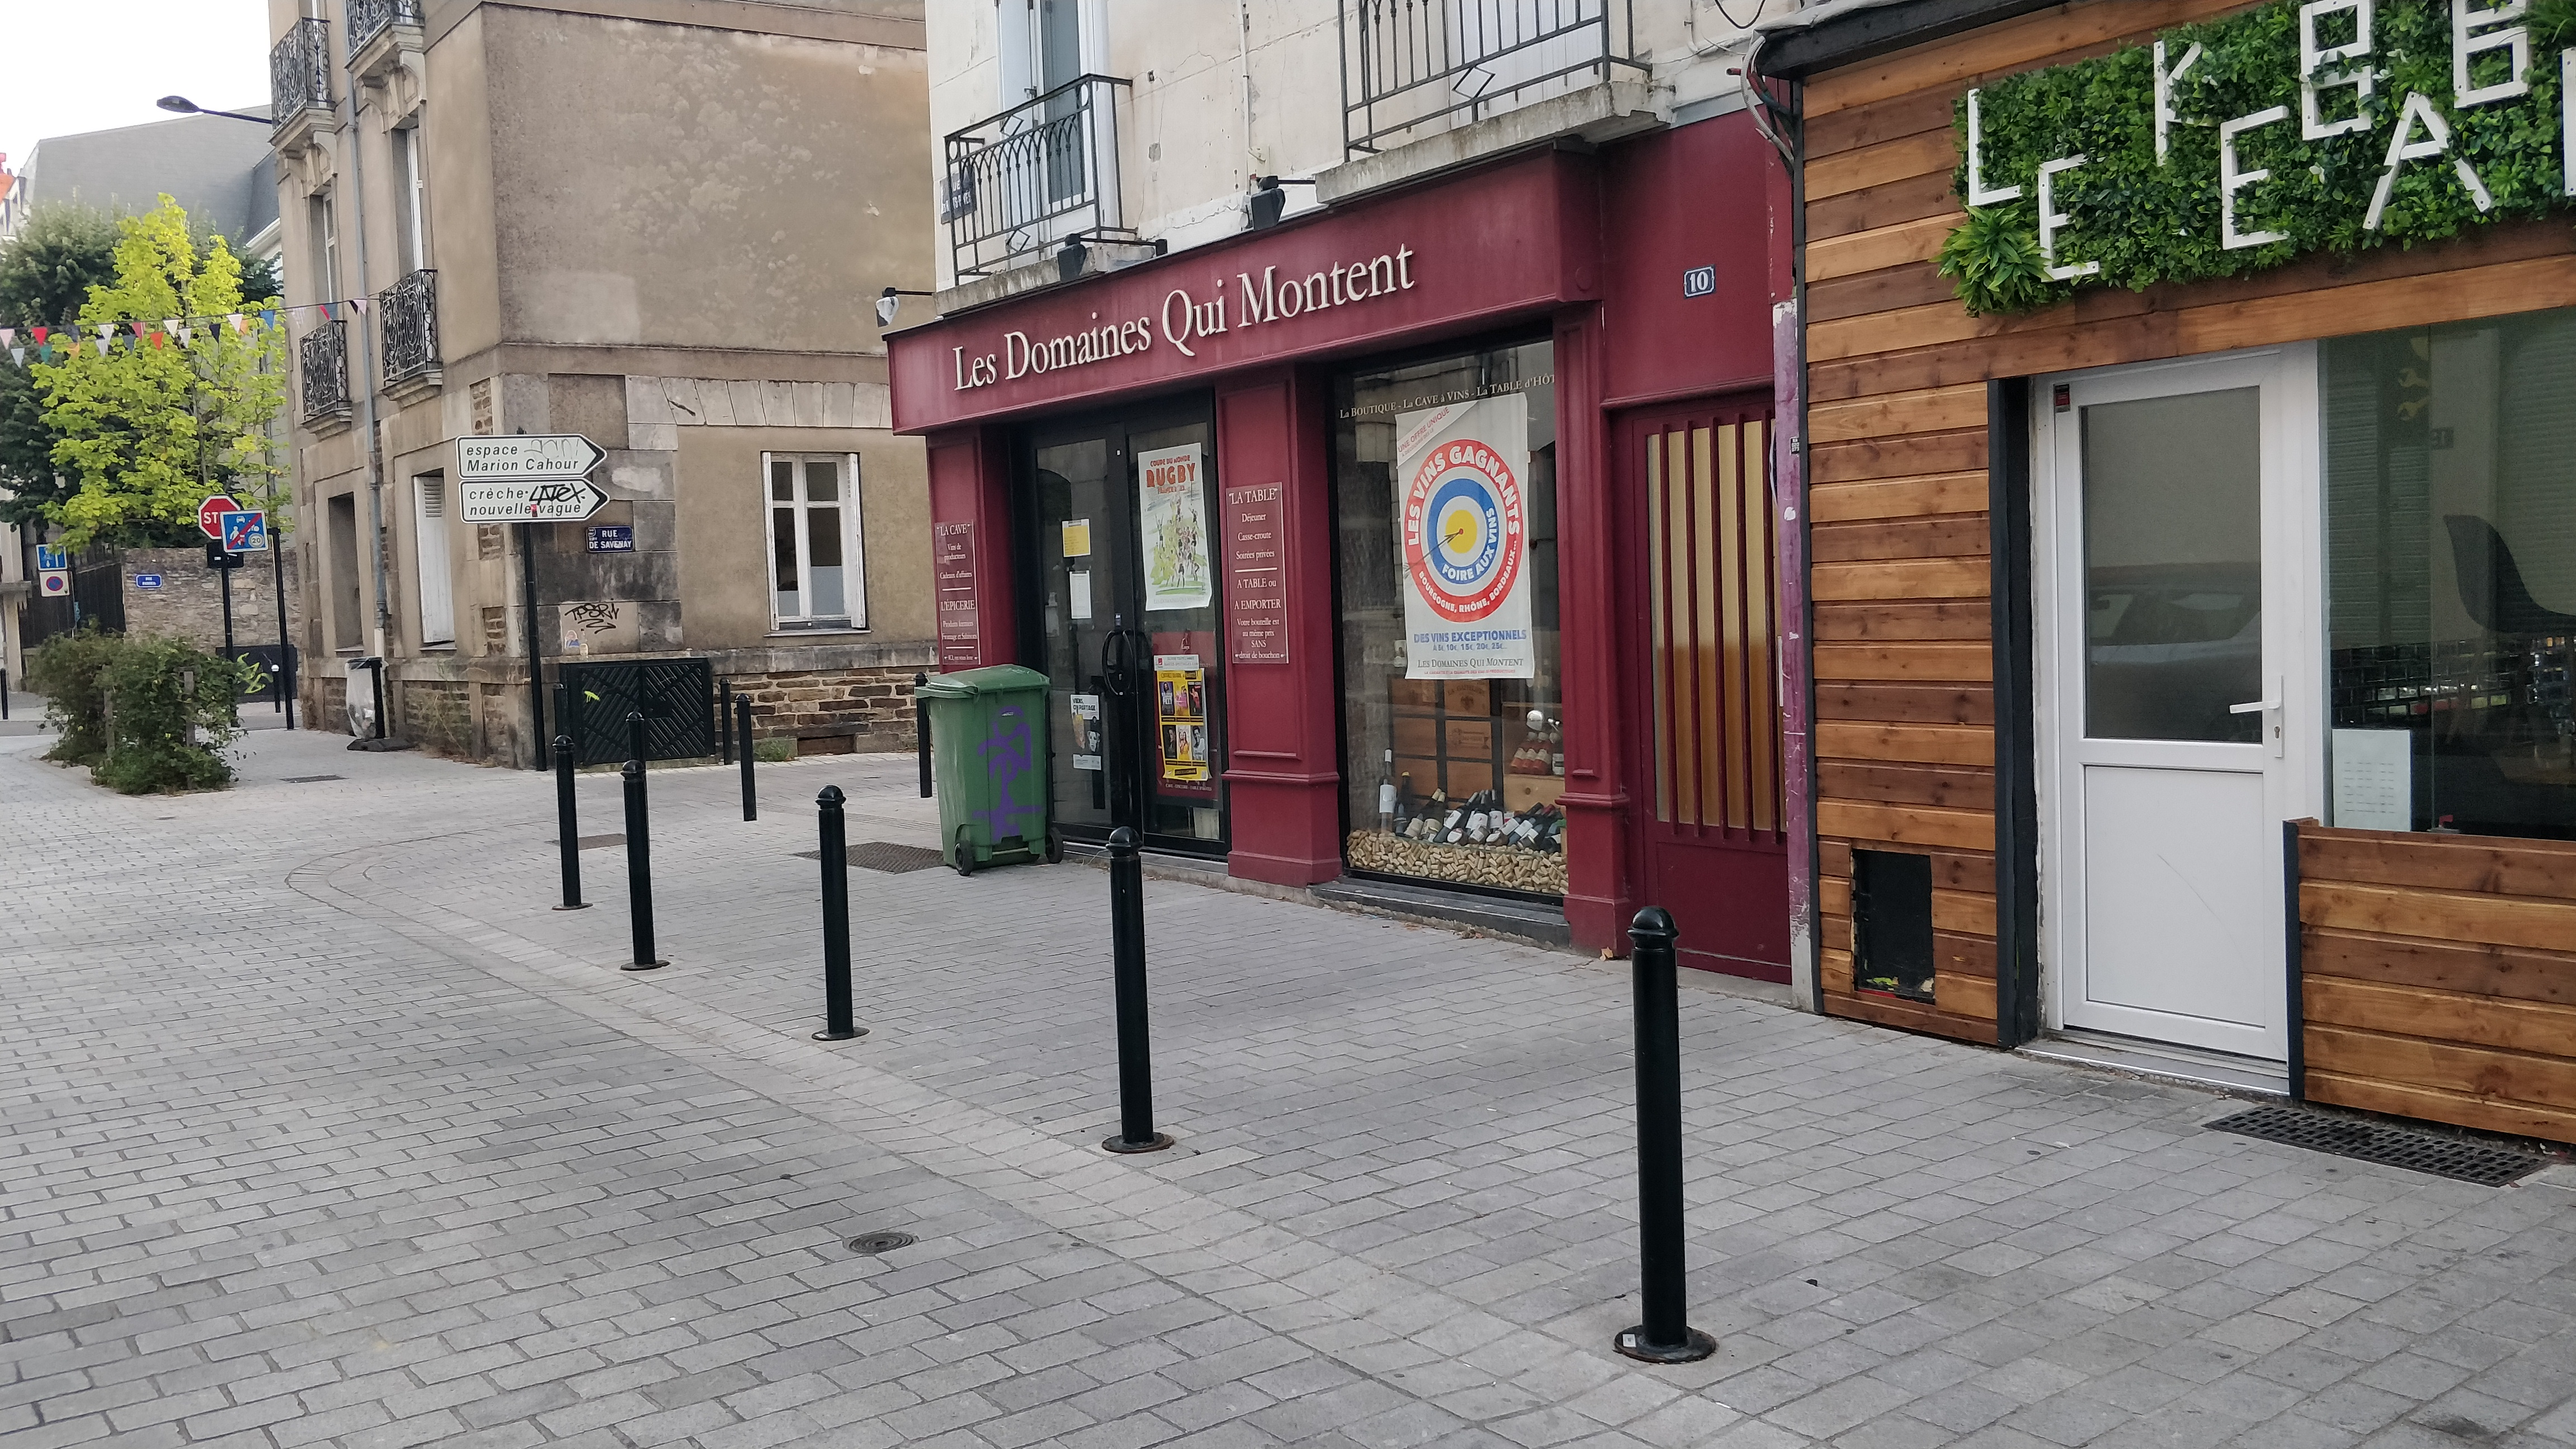
\includegraphics[width=0.7\textwidth]{images/IMG_20230914_075143-ped.jpg}
  \caption{Un trottoir au niveau de la chaussée : cette barrière
    prévient l'accès des voitures tout en garantissant une circulation
    fluide pour les piétons, y compris ceux à mobilité réduite, avec
    des poussettes ou accompagnés de jeunes enfants.}
  \label{fig:ped-flat}
\end{figure}

Malgré les rampes aux passages piétons, les trottoirs restent une
entrave pour beaucoup, surtout pour les personnes à mobilité réduite
et les parents avec poussettes. Leur déplacement est souvent
compliqué, limitant leur autonomie.

Nous plaidons pour une refonte de nos espaces urbains centrée sur
l’accessibilité. Plutôt que des trottoirs surélevés, envisageons des
bornes régulières le long des zones piétonnes (voir
figure~\ref{fig:ped-flat}). Ces bornes, tout en étant accessibles aux
piétons, bloqueraient l'accès aux voitures, garantissant ainsi la
sécurité.

Adopter cette vision c'est choisir une ville plus accessible,
sécurisée, et orientée vers l'humain. Nantes et les Pays de la Loire
doivent saisir cette opportunité pour le bien-être de tous leurs
citoyens.

